\documentclass{article}

\usepackage[english]{babel}

\usepackage[letterpaper,top=2cm,bottom=2cm,left=3cm,right=3cm,marginparwidth=1.75cm]{geometry}

% Useful packages
\usepackage{amsmath}
\usepackage{graphicx}
\usepackage[colorlinks=true, allcolors=blue]{hyperref}
\usepackage{listings}
\usepackage[T1]{fontenc}
\usepackage{textcomp}

\lstdefinestyle{bashStyle}{
  showstringspaces=false,
  language=bash,
  basicstyle=\small\sffamily,
  frame=tb,
  columns=fullflexible,
  linewidth=\linewidth,
  xleftmargin=0.075\linewidth,
  breaklines=true,
  literate =
    {'}{{\textquotesingle}}1
    {-}{{-}}1
}

\title{Modul 2 - Lambda for Image Optimization}
\author{}

\begin{document}
\lstset{language=Bash,upquote=true}
\begin{figure}[h]
\centering

\includegraphics[width=0.3\textwidth]{logo_lks_2023.jpg}
\end{figure}
\centering
{\huge
Lomba Kompetensi Siswa\\
Sekolah Menengah Kejuruan\\
Tingkat Provinsi Jawa Barat\\
Tahun 2023\\
\vspace{10mm} %5mm vertical space
}
\vspace{30mm} %5mm vertical space
{\let\newpage\relax\maketitle}
\vspace{30mm} %5mm vertical space
{\LARGE Bidang Lomba Cloud Computing}

\raggedright
\newpage

\section{Overview}
Optimizing images on a website is a critical aspect of enhancing user experience, reducing delivery costs, and boosting search engine rankings.
Given that images are typically the heaviest components of a web page in terms of both bytes and number of HTTP requests, it is important to implement effective optimization strategies.
Optimizing images can also enhance a website's search engine ranking, as demonstrated by Google's Largest Contentful Paint metric.
By implementing this solution, websites can achieve faster load times, lower costs, and improved visibility in search engine results.
You have been given a task to deploy an image optimizer solution on AWS. The API is built using AWS serverless components such as Amazon CloudFront, Amazon S3, and AWS Lambda. The solution requires to use a custom domain and an SSL.
\section{General Rules}
\begin{enumerate}
    \item Failure to comply with the rules will result in immediate disqualification.
    \item You have 3 hours to finish the tasks.
    \item You may not open any website unless otherwise specified in section \ref{references} and you may open the control panel of your domain provider to update the nameserver to Route 53.
    \item You may use AWS Console and AWS CLI to deploy the solutions. You may not use SAM, CloudFormation or CDK.
    \item Between and after the event, you may not access your account. Any activity on your AWS account during this period is not allowed.
    \item Resources should be given the least privilege. For example if a lambda function needs a put object permission to a bucket, then only give put object permission, do not give write object permission.
    \item During the event, multiple login is not permitted.
    \item If you have any question, do not hesitate to ask.
\end{enumerate}
\section{Architecture}\label{architecture}
\begin{figure}[h]
\centering
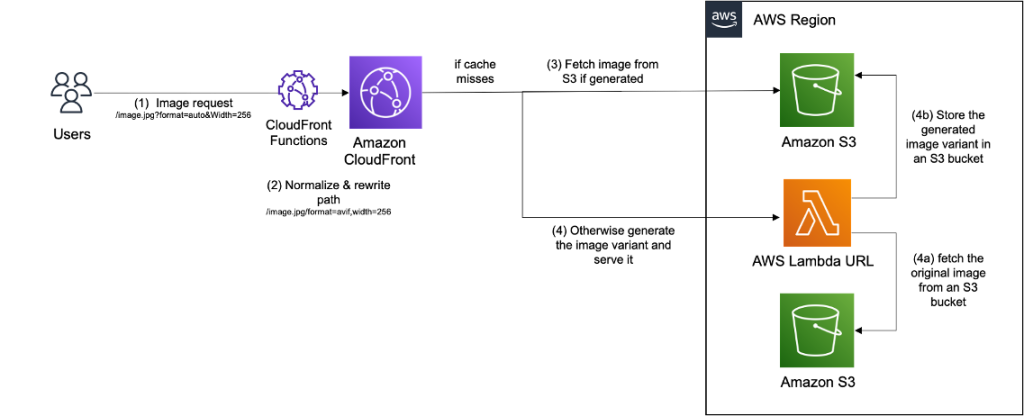
\includegraphics[width=\textwidth]{architecture.png}
\caption{\label{fig:architecture}Architecture Diagram}
\end{figure}

\begin{enumerate}
  \item A user requests an image with certain transformations, such as encoding and size, these transformations are encoded in the URL as query parameters. For instance, an example URL may look like this: \lstinline{https://example.com/images/01.jpg?format=webp&width=200.}
  \item The image request is initially handled by the nearest CloudFront edge location, ensuring optimal performance. A CloudFront Function is then executed on the viewer request event to rewrite the request URL before it is passed upstream. This function is designed for CDN customizations that require lightweight JavaScript functions capable of handling high-scale, latency-sensitive tasks. In our architecture, the URL is rewritten to validate the requested transformations, normalize the URL by ordering transformations and converting them to lower case, thus increasing the cache hit ratio. Additionally, when an automatic transformation is requested, the function determines the best one to apply. For example, if the user specifies the "format=auto" directive for the most optimized image format (JPEG, WebP, or AVIF), the CloudFront Function selects the optimal format based on the Accept header present in the request.
  \item When a user requests an image that is already cached in CloudFront, the image is immediately returned from the CloudFront cache, resulting in a cache hit. However, if the image is not present in the CloudFront cache, the request is forwarded to an S3 bucket created specifically for storing transformed images. If the requested image has already been transformed and stored in S3, it is served and cached in CloudFront, with no need for further transformation.
  \item If the requested image does not exist in the bucket for the transformed images, S3 will respond with a 403 error code. CloudFront's Origin Failover feature detects this error and retries the same URL, but this time using the secondary origin based on the Lambda function URL. The Lambda function is then invoked and downloads the original image from a separate S3 bucket where the original images are stored. Using the Sharp library, the Lambda function transforms the image, stores it in S3, and serves it through CloudFront, where it is cached for future requests.
\end{enumerate}

\section{Information}

\begin{enumerate}
\item The repository URL for the required source code to deploy this solution is \href{https://github.com/kensasongko/lksccjabar2023modul2_aplikasi}{https://github.com/kensasongko/lksccjabar2023modul2\_aplikasi}
\item This solution must be deployed in \textbf{ap-southeast-1 (Singapore) region}. Deploying in another region will result in a major point reduction.
\end{enumerate}

\section{Task}
Your task is to create the solution from the section \ref{architecture}.
\begin{enumerate}
\item Create 2 S3 buckets, one to store the original images and another one to store the transformed images.
  \begin{itemize}
    \item Original image bucket:
    \begin{itemize}
      \item Add a tag to the bucket: Key=LKS-ID, Value=MODUL2-ORIGINAL
    \end{itemize}
    \item Transformed image bucket:
    \begin{itemize}
      \item Create a lifecycle policy to remove images after 30 days.
      \item Add a tag to the bucket: Key=LKS-ID, Value=MODUL2-TRANSFORMED
    \end{itemize}
    \item Both buckets should have the following configuration:
    \begin{itemize}
      \item Enable block all public access.
      \item Access: Bucket and objects not public
    \end{itemize}
  \end{itemize}
\item Deploy lambda:
  \begin{itemize}
    \item Install Sharp
    \item Create a development package from the image-processing directory.
    \item Create and deploy the lambda function with the following configuration:
    \begin{itemize}
      \item Lambda runtime: nodejs16.x
      \item Memory size: 512 MB
      \item Give the function policies as stated in the README.md.
      \item Add environment variables as stated in the README.md.
      \item Create function URL with Auth Type = None.
      \item Add a tag to the function: Key=LKS-ID, Value=MODUL2
    \end{itemize}
    \item Check README.md for more instruction.
  \end{itemize}
\item Create a certificate for *.[YOUR\_DOMAIN] in ACM for CloudFront.
\item Create a CloudFront distribution with the following configuration:
  \begin{itemize}
    \item Price class: Use all edge locations (best performance)
    \item Supported HTTP versions: HTTP/2
    \item Viewer protocol policy: Redirect HTTP to HTTPS
    \item Security policy: TLSv1.2\_2021
    \item Standard logging: Off
    \item Cookie logging: Off
    \item Alternate domain name: https://modul2.[YOUR\_DOMAIN]
    \item Cache Policy:
    \begin{itemize}
      \item TTL Settings - Minimum TTL (seconds): 10
      \item TTL Settings - Maximum TTL (seconds): 31536000
      \item TTL Settings - Default TTL (seconds): 86400
      \item Cache Keys - Headers: None
      \item Cache Keys - Cookies: None
      \item Cache Keys - Query strings: All
      \item Compression support - Gzip: Disabled
      \item Compression support - Brotli: Disabled
    \end{itemize}
    \item Response headers policy:
    \begin{itemize}
      \item Cross-origin resource sharing (CORS) - Access-Control-Allow-Credentials: False
      \item Cross-origin resource sharing (CORS) - Access-Control-Allow-Headers: *
      \item Cross-origin resource sharing (CORS) - Access-Control-Allow-Methods: GET
      \item Cross-origin resource sharing (CORS) - Access-Control-Allow-Origin: *
      \item Cross-origin resource sharing (CORS) - Access-Control-Expose-Headers: -
      \item Cross-origin resource sharing (CORS) - Access-Control-Max-Age (seconds): 600
    \end{itemize}
    \item Create an origin group which contains of 2 origins (failover criteria: 403) as explained in section \ref{architecture}. The first origin is the transformed bucket, the second origin is the lambda function URL. Add a custom header to the second origin, the name of the custom header is x-origin-secret-header and, the value is the secrey key you have previously added to the lambda function.
    \item Add a tag to the distribution: Key=LKS-ID, Value=MODUL2
  \end{itemize}
  \item Create a CloudFront function from the url-rewrite directory and add it to Viewer request function of the CloudFront distribution.
\end{enumerate}
\section{How to test your deployment}
\begin{enumerate}
  \item Upload an image to the original image bucket (this example uses test1.png as the test image)
  \item Using your browser open http://modul2.[YOUR\_DOMAIN]/test1.png.
  \item Check whether /test1.png/original exists in your transformed bucket image.
  \item Using your browser open http://modul2.[YOUR\_DOMAIN]/test1.png?width=200.
  \item Check whether /test1.png/width=200 exists in your transformed bucket image.
\end{enumerate}
\section{References}\label{references}
\begin{itemize}
  \item \href{https://docs.aws.amazon.com/AmazonS3/latest/userguide/Welcome.html}{S3 documentation}
  \item \href{https://docs.aws.amazon.com/lambda/latest/dg/welcome.html}{Lambda documentation}
  \item \href{https://docs.aws.amazon.com/Route53/latest/DeveloperGuide/Welcome.html}{Route 53 documentation}
  \item \href{https://docs.aws.amazon.com/acm/latest/userguide/acm-overview.html}{Certificate Manager documentation}
  \item \href{https://docs.aws.amazon.com/AmazonCloudFront/latest/DeveloperGuide/Introduction.html}{CloudFront documentation}
  \item \href{https://sharp.pixelplumbing.com/}{Sharp documentation}
  \item \href{https://docs.npmjs.com/}{NPM documentation}
\end{itemize}
\section*{Good luck!}

\end{document}
